\documentclass[runningheads]{llncs}

% ECCV 2026 review style (TODO FINAL: swap to \usepackage{eccv} for camera-ready).
\usepackage[review,year=2026,ID=*****]{eccv}
\usepackage{eccvabbrv}
\usepackage{graphicx}
\usepackage{booktabs}
\usepackage{subcaption}
\usepackage{multirow}

% Unicode passthrough (raw glyphs for degrees / math / accents).
\usepackage{newunicodechar}
\newunicodechar{°}{\ensuremath{^\circ}}\newunicodechar{×}{\ensuremath{\times}}\newunicodechar{–}{--}\newunicodechar{—}{---}
\newunicodechar{↔}{\ensuremath{\leftrightarrow}}\newunicodechar{δ}{\ensuremath{\delta}}\newunicodechar{α}{\ensuremath{\alpha}}
\newunicodechar{≈}{\ensuremath{\approx}}\newunicodechar{→}{\ensuremath{\rightarrow}}\newunicodechar{≤}{\ensuremath{\le}}
\newunicodechar{≥}{\ensuremath{\ge}}\newunicodechar{≪}{\ensuremath{\ll}}\newunicodechar{≫}{\ensuremath{\gg}}\newunicodechar{·}{\ensuremath{\cdot}}
\newunicodechar{∈}{\ensuremath{\in}}\newunicodechar{±}{\ensuremath{\pm}}\newunicodechar{−}{\ensuremath{-}}\newunicodechar{≠}{\ensuremath{\neq}}
\newunicodechar{“}{``}\newunicodechar{”}{''}\newunicodechar{‘}{`}\newunicodechar{’}{'}\newunicodechar{Δ}{\ensuremath{\Delta}}\newunicodechar{★}{\ensuremath{\star}}\newunicodechar{∼}{\ensuremath{\sim}}
\newunicodechar{é}{\'e}\newunicodechar{è}{\`e}\newunicodechar{ê}{\^e}\newunicodechar{ô}{\^o}\newunicodechar{ö}{\"o}\newunicodechar{ü}{\"u}\newunicodechar{ä}{\"a}\newunicodechar{á}{\'a}\newunicodechar{ñ}{\~n}\newunicodechar{ç}{\c{c}}

\usepackage{hyperref}
% AUTO-GENERATED by scripts/emit_paper_tex.py from results/metrics/paper_data.json. DO NOT EDIT.
% git ec6ae88  config 07bca1207c0a  fast=False
\newcommand{\HumanTFPone}{0.49}
\newcommand{\HumanTFPend}{0.93}
\newcommand{\HumanNumFixTP}{3}
\newcommand{\HumanNumFixTA}{5}
\newcommand{\HumanNumFixTAmax}{45}
\newcommand{\HumanCeiling}{0.53}
\newcommand{\HumanDprime}{2.91}
\newcommand{\NImages}{285}
\newcommand{\NImagesTP}{141}
\newcommand{\NImagesTA}{144}
\newcommand{\NSeeds}{5}
\newcommand{\PCApcone}{45}
\newcommand{\PCApctwo}{30}
\newcommand{\NEpisodes}{38{,}475}
\newcommand{\QwenTPexist}{0.99}
\newcommand{\QwenTAexist}{0.81}
\newcommand{\QwenYesBias}{0.19}
\newcommand{\QwenLocaliz}{0.00}
\newcommand{\QwenSharpTFPone}{0.97}
\newcommand{\QwenSharpTFPend}{0.97}
\newcommand{\QwenSharpNumFixTP}{2}
\newcommand{\QwenSharpNumFixTA}{1}
\newcommand{\QwenSharpDeclAbs}{0.94}
\newcommand{\QwenSharpFalsePresent}{0.06}
\newcommand{\QwenSharpDprime}{3.66}
\newcommand{\QwenSharpEntropyD}{$-$.68}
\newcommand{\QwenSharpSaccD}{$+$.52}
\newcommand{\QwenSharpCenterD}{$-$.20}
\newcommand{\QwenSharpSelfConsist}{0.84}
\newcommand{\QwenSharpScanmatchAH}{0.50}
\newcommand{\QwenSharpDensityCC}{0.55}
\newcommand{\QwenGPTFPone}{0.97}
\newcommand{\QwenGPTFPend}{0.98}
\newcommand{\QwenGPNumFixTP}{2}
\newcommand{\QwenGPNumFixTA}{1}
\newcommand{\QwenGPDeclAbs}{0.93}
\newcommand{\QwenGPFalsePresent}{0.07}
\newcommand{\QwenGPDprime}{3.84}
\newcommand{\QwenGPEntropyD}{$-$.67}
\newcommand{\QwenGPSaccD}{$+$.50}
\newcommand{\QwenGPCenterD}{$-$.18}
\newcommand{\QwenGPSelfConsist}{0.84}
\newcommand{\QwenGPScanmatchAH}{0.50}
\newcommand{\QwenGPDensityCC}{0.58}
\newcommand{\QwenKsixteenTFPone}{0.78}
\newcommand{\QwenKsixteenTFPend}{0.91}
\newcommand{\QwenKtwentyfourTFPone}{0.56}
\newcommand{\QwenKtwentyfourTFPend}{0.81}
\newcommand{\QwenKthirtytwoTFPone}{0.42}
\newcommand{\QwenKthirtytwoTFPend}{0.71}
\newcommand{\QwenNumFixCIzero}{no}
\newcommand{\QwenNumFixDelta}{-1.49}
\newcommand{\GlmTPexist}{0.99}
\newcommand{\GlmTAexist}{0.81}
\newcommand{\GlmYesBias}{0.19}
\newcommand{\GlmLocaliz}{0.31}
\newcommand{\GlmSharpTFPone}{0.97}
\newcommand{\GlmSharpTFPend}{0.98}
\newcommand{\GlmSharpNumFixTP}{2}
\newcommand{\GlmSharpNumFixTA}{4}
\newcommand{\GlmSharpDeclAbs}{0.91}
\newcommand{\GlmSharpFalsePresent}{0.03}
\newcommand{\GlmSharpDprime}{4.09}
\newcommand{\GlmSharpEntropyD}{$-$.65}
\newcommand{\GlmSharpSaccD}{$+$.60}
\newcommand{\GlmSharpCenterD}{$-$.29}
\newcommand{\GlmSharpSelfConsist}{0.90}
\newcommand{\GlmSharpScanmatchAH}{0.48}
\newcommand{\GlmSharpDensityCC}{0.54}
\newcommand{\GlmGPTFPone}{0.97}
\newcommand{\GlmGPTFPend}{0.98}
\newcommand{\GlmGPNumFixTP}{2}
\newcommand{\GlmGPNumFixTA}{4}
\newcommand{\GlmGPDeclAbs}{0.91}
\newcommand{\GlmGPFalsePresent}{0.03}
\newcommand{\GlmGPDprime}{4.23}
\newcommand{\GlmGPEntropyD}{$-$.65}
\newcommand{\GlmGPSaccD}{$+$.61}
\newcommand{\GlmGPCenterD}{$-$.31}
\newcommand{\GlmGPSelfConsist}{0.91}
\newcommand{\GlmGPScanmatchAH}{0.48}
\newcommand{\GlmGPDensityCC}{0.63}
\newcommand{\GlmKsixteenTFPone}{0.71}
\newcommand{\GlmKsixteenTFPend}{0.80}
\newcommand{\GlmKtwentyfourTFPone}{0.49}
\newcommand{\GlmKtwentyfourTFPend}{0.65}
\newcommand{\GlmKthirtytwoTFPone}{0.33}
\newcommand{\GlmKthirtytwoTFPend}{0.53}
\newcommand{\GlmNumFixCIzero}{no}
\newcommand{\GlmNumFixDelta}{-1.60}
\newcommand{\GemmaTPexist}{0.97}
\newcommand{\GemmaTAexist}{0.80}
\newcommand{\GemmaYesBias}{0.20}
\newcommand{\GemmaLocaliz}{0.87}
\newcommand{\GemmaSharpTFPone}{0.80}
\newcommand{\GemmaSharpTFPend}{0.93}
\newcommand{\GemmaSharpNumFixTP}{3}
\newcommand{\GemmaSharpNumFixTA}{6}
\newcommand{\GemmaSharpDeclAbs}{0.96}
\newcommand{\GemmaSharpFalsePresent}{0.03}
\newcommand{\GemmaSharpDprime}{3.11}
\newcommand{\GemmaSharpEntropyD}{$-$.28}
\newcommand{\GemmaSharpSaccD}{$+$.24}
\newcommand{\GemmaSharpCenterD}{$+$.06}
\newcommand{\GemmaSharpSelfConsist}{0.71}
\newcommand{\GemmaSharpScanmatchAH}{0.47}
\newcommand{\GemmaSharpDensityCC}{0.49}
\newcommand{\GemmaGPTFPone}{0.80}
\newcommand{\GemmaGPTFPend}{0.93}
\newcommand{\GemmaGPNumFixTP}{3}
\newcommand{\GemmaGPNumFixTA}{5}
\newcommand{\GemmaGPDeclAbs}{0.96}
\newcommand{\GemmaGPFalsePresent}{0.02}
\newcommand{\GemmaGPDprime}{3.14}
\newcommand{\GemmaGPEntropyD}{$-$.27}
\newcommand{\GemmaGPSaccD}{$+$.23}
\newcommand{\GemmaGPCenterD}{$+$.06}
\newcommand{\GemmaGPSelfConsist}{0.71}
\newcommand{\GemmaGPScanmatchAH}{0.47}
\newcommand{\GemmaGPDensityCC}{0.50}
\newcommand{\GemmaKsixteenTFPone}{0.42}
\newcommand{\GemmaKsixteenTFPend}{0.75}
\newcommand{\GemmaKtwentyfourTFPone}{0.28}
\newcommand{\GemmaKtwentyfourTFPend}{0.65}
\newcommand{\GemmaKthirtytwoTFPone}{0.19}
\newcommand{\GemmaKthirtytwoTFPend}{0.59}
\newcommand{\GemmaNumFixCIzero}{yes}
\newcommand{\GemmaNumFixDelta}{-0.03}
              % numeric macros (auto-generated; do not edit by hand)

\begin{document}

\title{Matched Outcomes, Divergent Gaze: How Foveated MLLMs Search Compared to Humans \thanks{The recorded data and the analysis code required to reproduce every result will be released upon publication.}}

\titlerunning{Matched Outcomes, Divergent Gaze}
\author{Anonymous ECCV 2026 submission}
\authorrunning{Anonymous ECCV 2026 submission}
\institute{Paper ID *****}
\maketitle



\begin{abstract}
Human visual search is \emph{serial}: the fovea must land on a candidate to confirm it, producing a
scanpath. Whether multimodal large language models (MLLMs), constrained to the same foveated input, search
as humans do bears on their use as models of human vision and on attention-alignment scores. Three
general-purpose MLLMs are compared with human eye-movement scanpaths on goal-directed search
(COCO-Search18), each driven fixation-by-fixation through an identical human-matched foveated view and
assessed along three axes: the \emph{decision} (target present or absent), the \emph{efficiency} of
reaching the target, and the \emph{gaze process} itself. The axes dissociate. On the decision and on
target acquisition the models match or exceed humans, detecting present targets near ceiling and reaching them on
the first saccade more often than humans. The gaze process is not human: all three share one
signature---low-entropy, large-amplitude, self-consistent scanpaths that agree with themselves far more
closely than two humans agree. This is consistent with a single-pass, non-serial architecture rather than
a limit of acuity: matched retinal input reproduces where humans look but not how looking unfolds, and no
degree of peripheral degradation recovers human-like search. The difference lies on a process axis that
answer-alignment and saliency metrics do not measure; such metrics cannot certify human-like vision, and
zero-shot models suit outcome and spatial questions, not temporal, process-level ones.
  \keywords{Visual search \and Foveated vision \and Multimodal LLMs \and Eye movements
  \and COCO-Search18 \and Human-model alignment}
\end{abstract}




\section{Introduction}

Human goal-directed visual search is a \emph{serial} process. The fovea resolves fine detail only within
$\sim$1--2$^{\circ}$ of gaze, so a target detected coarsely in the periphery must be fixated before it can
be confirmed; search unfolds as a sequence of saccades whose targeting, extent and termination are well
characterised, theoretically \cite{heaton2020serial,gupta2022asymmetry}, computationally
\cite{bujia2022bayes,travi2022bench,yang2020irl,yang2024hat}, and empirically on datasets such as
COCO-Search18 for target-present and target-absent search \cite{chen2021cocosearch18,chen2022targetabsent}.
This seriality is imposed by the optics of the eye and is what a foveated agent must pay to search.

This motivates a falsifiable hypothesis: if a model views a scene through the \emph{same} foveated,
acuity-limited aperture as a human---sharp at gaze, degraded in the periphery, displaceable only by
re-fixating---then matched retinal input ought to induce matched search behaviour. The assumption is
load-bearing for two common practices: using multimodal large language models (MLLMs) as stand-ins for
human observers, and reading attention-alignment scores (the overlap between model attention and human
fixations) as evidence that a model ``sees like us''. Both take behavioural or spatial agreement to
license a claim about \emph{process}. We test this by decomposing ``human-like search'' into three axes and
asking on which, if any, an MLLM resembles a human: \emph{decision} (target present or absent?),
\emph{finding} (does gaze reach the target, at what cost?), and \emph{gaze} (are the eye-movement dynamics
human-like?). Three general-purpose MLLMs from three families (Qwen3.5-35B-A3B~\cite{qwen3.5}, GLM-4.6V-Flash~\cite{vteam2025glm45vglm41vthinkingversatilemultimodal},
Gemma-4-E4B~\cite{gemmateam2026gemma4technicalreport}) search COCO-Search18 fixation-by-fixation through a byte-identical foveation harness, against
ten human scanpaths per scene.

The axes \emph{dissociate} (Fig.~\ref{fig:diss}). On decision and finding the models are
human-or-better---near-ceiling present-target detection and first-saccade target fixation
\QwenGPTFPone/\GlmGPTFPone/\GemmaGPTFPone\ versus the human \HumanTFPone, at comparable eventual success and
no more fixations---yet on gaze they are non-human, the three sharing \emph{one} low-entropy,
large-amplitude, highly self-consistent signature that agrees with itself far more than with any human
(cross-seed ScanMatch \QwenGPSelfConsist/\GlmGPSelfConsist/\GemmaGPSelfConsist\ against the inter-observer
ceiling \HumanCeiling). The correct outcome is produced by a shared, non-human process---consistent with a
single-pass, non-serial architecture rather than a limit of acuity, as matched retinal \emph{input}
reproduces \emph{where} humans look but not \emph{how} looking unfolds (\S\ref{sec:gaze}). Our contributions
follow: answer-alignment and saliency metrics are blind to this process axis and cannot certify human-like
vision; zero-shot MLLMs suit outcome and spatial questions but not process and temporal ones; and a
non-serial searcher that matches human outcomes is a null model for the human serial bottleneck. We do not
propose a scanpath predictor or compete on accuracy.

\section{Related work}

\textbf{Human search and its models.} COCO-Search18 provides laboratory human fixations for target-present
and target-absent search \cite{chen2021cocosearch18,chen2022targetabsent} and anchors scanpath
predictors---inverse-reinforcement-learning and transformer models
\cite{yang2020irl,yang2024hat,mondal2023gazeformer} and ideal-observer/Bayesian searchers benchmarked on
common data \cite{bujia2022bayes,travi2022bench}. Classically, search mixes parallel peripheral evaluation
with serial focal inspection \cite{heaton2020serial}, and search asymmetries emerge from natural-image
statistics rather than task-specific training \cite{gupta2022asymmetry}. These \emph{predict or explain
human} attention; we characterise an MLLM's \emph{process} against the same reference, taking seriality as
the property we test.

\textbf{Foveation as a modelling constraint.} The Geisler--Perry acuity fall-off \cite{geisler1998foveation}
supplies our human-matched renderer. Foveated-observer models capture human performance that non-foveated
metrics miss---medical search \cite{lago2021foveated}, foveated transformers \cite{jonna2022foveatedvit},
scene-understanding time \cite{wen2025fsum}, dual ``what''/``where'' saccade selection
\cite{dauce2020dual}---and semantically guided foveal models predict human scanpaths on COCO-Search18
\cite{luzio2024semantic,luzio2025semba}. Most pointedly, biologically constrained networks viewing scenes
foveally produce human-like scanpaths \emph{without being trained to} \cite{neva,nevaclip}. That foveation
has repeatedly \emph{sufficed} to induce human-like search motivates our question; for a general-purpose
MLLM it does not (Sec.~4.3).

\textbf{MLLM versus human vision.} A growing literature asks whether MLLMs perceive as humans
do---cognitive paradigms \cite{burden2025ispy,lin2024hvsbench,blink,tet}, which find that models ``see but do
not perceive'', and attention comparison via eye-tracking \cite{ghamati2025whichai,soodMRC,vqamhug} where
attention similarity and task performance dissociate \cite{soodMRC}; critiques of linguistic-prior reliance
separate spatial from semantic guidance \cite{kanade2025doyousee,wu2025indoor}. Closest, MLLM competence
and the human process come apart: a serial deficit inferred from reaction time \cite{budny}, human-trivial
search on which VLMs barely beat chance \cite{berman2025tunnelvision}, correct region with wrong answer
\cite{knowwheretolook}---the mirror of our right-answer/non-human-process finding, but on a static
map---and a capability--strategy gap accuracy benchmarks miss \cite{bayesbench}. We differ in measuring the
fixation-by-fixation process, with an explicit stopping decision, on an axis these do not assess.

\textbf{Agentic, search-trained MLLMs.} A parallel line adds active perception to raise accuracy---LLM-guided
search \cite{wu2023vstar}, tree-based zoom \cite{shen2024zoomeye}, reinforcement-learned focusing
\cite{bai2026glanceorgaze,lai2025minio3,li2025insighto3}, and embodied variants \cite{hstar360,mllmsearch};
chain-of-thought can even \emph{degrade} an embodied searcher \cite{vlnmme}. These optimise \emph{what} is
answered by learning \emph{where} to look. We instead characterise \emph{how} a general-purpose model
explores under a fixed foveation constraint, without search-specific training; trained agents are the most
pertinent next comparison (Sec.~\ref{sec:lim}) but out of scope.


 
\begin{figure}[t]\centering
  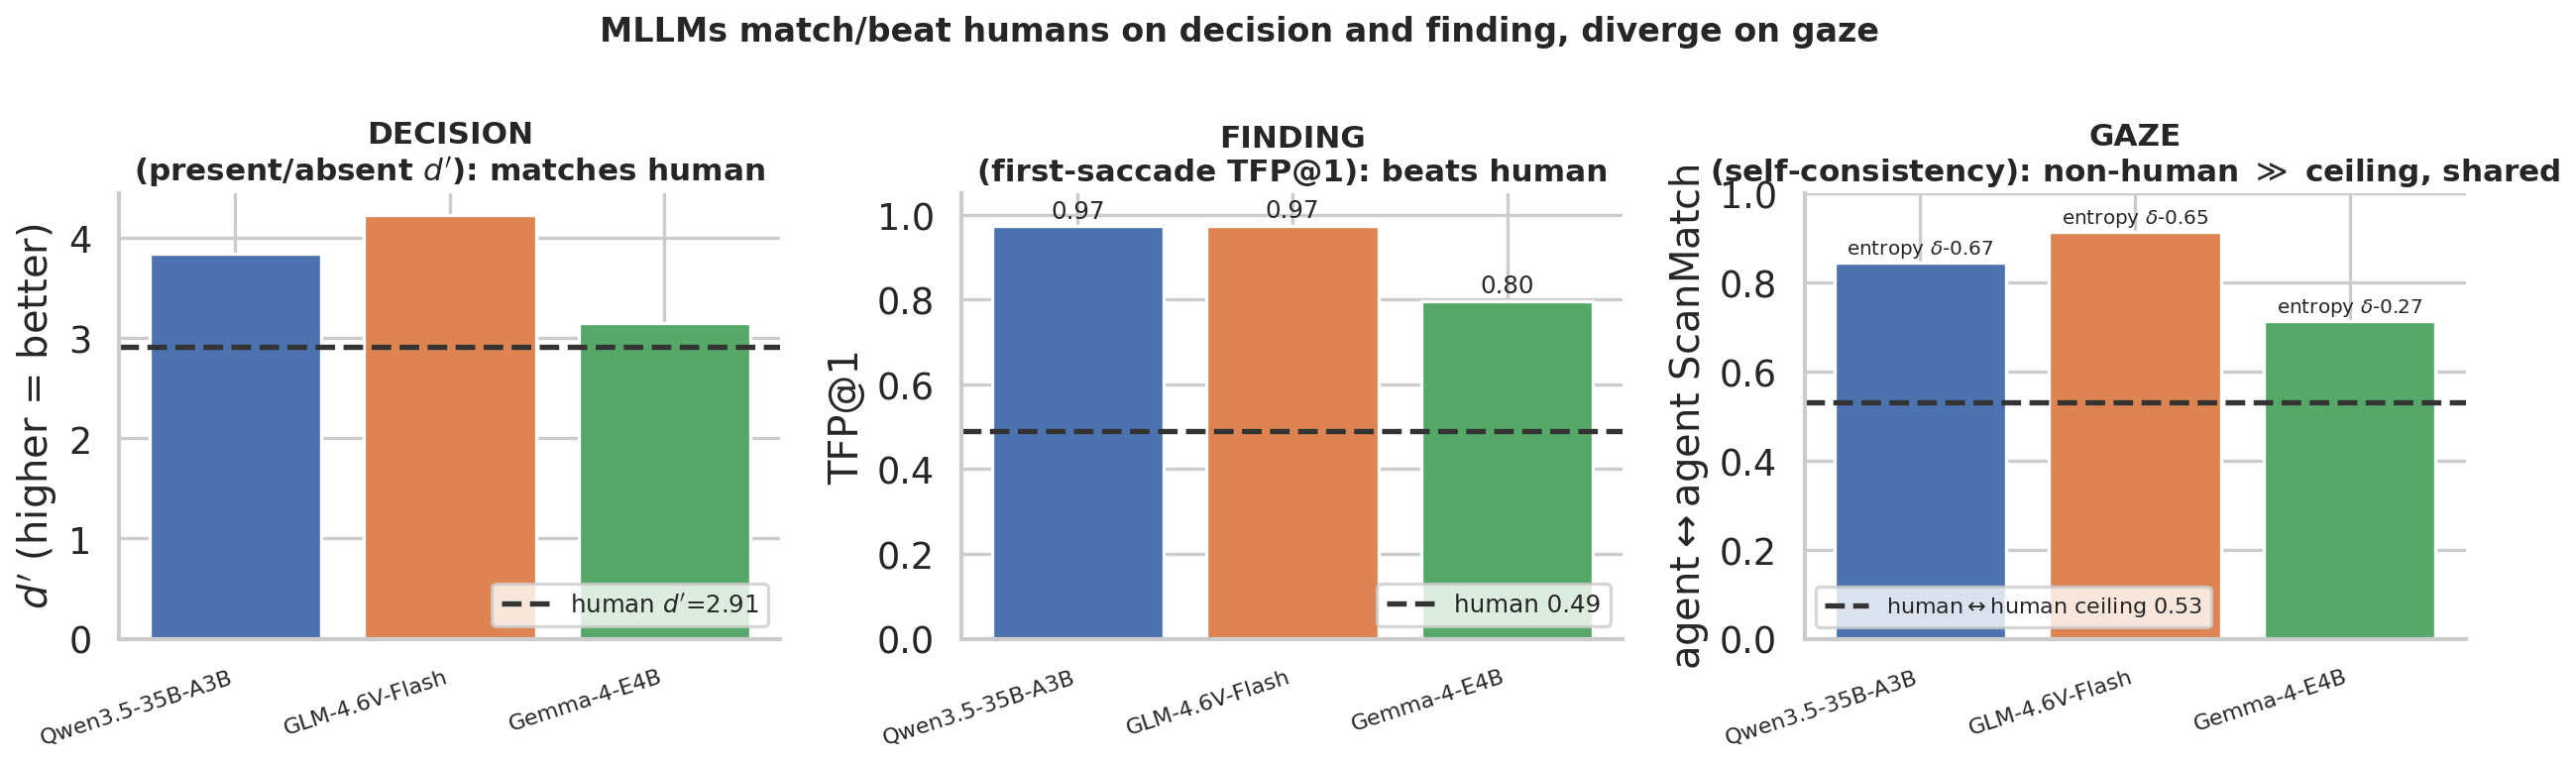
\includegraphics[width=\linewidth]{figures/fig_dissociation.png}
  \caption{The three-axis dissociation at the human-matched condition. \emph{Decision} ($d'$,
  present/absent): the models match or exceed the human reference. \emph{Finding} (first-saccade TFP@1): the models
  exceed the human rate (\HumanTFPone) by a wide margin. \emph{Gaze} (cross-seed self-consistency): all
  three lie above the human$\leftrightarrow$human ceiling (\HumanCeiling) and apart from the human
  (bar height, cross-seed ScanMatch; annotation, gaze-entropy Cliff's $\delta$), with Gemma-4-E4B nearest. The correct outcome is produced by a shared,
  non-human process.}
  \label{fig:diss}
   \vspace{-7mm}
\end{figure}

 



  \vspace{-5mm}
\section{Method}
 \vspace{-3mm}
\textbf{Data.} The human reference is COCO-Search18~\cite{chen2021cocosearch18}: ten observers per scene
issuing a gamepad present/absent decision on $1680{\times}1050$\,px scenes subtending $\sim$$54°{\times}35°$
($\to\sim$$30$\,px/deg). We use the validation split and a frozen, category-stratified subset of
\NImagesTP\ target-present and \NImagesTA\ target-absent scenes (all ten human scanpaths each); the unit
of analysis is the (scene, target) trial. \textbf{Foveation bracket.} At the gaze point a deterministic
renderer applies one of four condition \emph{families} (nine conditions in total; Fig.~\ref{fig:bracket}): \textsc{sharp}; \textsc{geisler--perry}
(GP), the Geisler and Perry~\cite{geisler1998foveation} acuity falloff (the only human-matched
condition; its mild appearance reflects that peripheral information at this viewing geometry is more legible than intuition suggests, and follows the calibrated falloff of Sec.~S1); \textsc{gaussian} ``gist-$k$'' (``gist'' denotes the coarse peripheral information surviving foveation), the same falloff with peripheral
acuity reduced by $k\in\{8,16,24,32,48,128\}$ (a synthetic degradation not tuned to human behaviour); and
\textsc{crop}, a fovea-only disc. \textbf{Procedure.} Each episode begins at a forced central fixation; at
every step the model observes the scene rendered at its gaze point (earlier glimpses retained in context)
and returns one directive: \textsc{look}, \textsc{found}, or \textsc{absent}. We use ``scanpath''/``gaze'' for the model's sequence of requested fixation coordinates: an operational analogue of oculomotor scanning, not a claim that the model has eye movements. No search policy is
imposed; the $50$-glimpse cap never forces termination (episodes end on the model's own \textsc{found}/\textsc{absent} decision). Decisions use a single free-form
generation per step at temperature $0.6$ under \NSeeds\ seeds; the harness, prompt (see the supplementary material) and renderer are identical across models. The Geisler--Perry falloff is computed in the native $1680{\times}1050$ frame and each glimpse is then downscaled uniformly to a $1024$-px maximum side, preserving the falloff geometry up to a global scale. \textbf{Models.} Qwen3.5-35B-A3B (a 35B mixture-of-experts, 3B active;
reasoning-tuned), GLM-4.6V-Flash ($\approx$$9$B; reasoning-tuned) and Gemma-4-E4B ($\approx$$4$B;
instruction-tuned, run with thinking disabled), which differ in architecture, family and training recipe; as these factors covary,
any cross-model trend is reported descriptively.\footnote{HuggingFace checkpoints \texttt{Qwen/Qwen3.5-35B-A3B}, \texttt{zai-org/GLM-4.6V-Flash}, \texttt{google/gemma-4-E4B-it}. The two reasoning-tuned models run with their default thinking and Gemma-4-E4B with thinking disabled; at each step only the final directive line is consumed.} \textbf{Measures.} Search is interpreted only on trials
passing the one-shot existence test, whose detection ceiling is near-identical across models
(Sec.~\ref{sec:dec}). We report, for \emph{decision}, existence accuracy and signal-detection $d'$ (criterion in Sec.~S4); for \emph{finding}, target-fixation probability (TFP) by saccade, with a hit defined as a
fixation within $1°$ of the target box, and fixation count; and for \emph{gaze}, the per-scanpath signature
(saccade amplitude, entropy, refixation, length, center bias, turning angle, coverage) as Cliff's $\delta$
against humans, scanpath
similarity~\cite{cristino2010scanmatch} against the human$\leftrightarrow$human
ceiling, and a cross-model PCA. All measures are defined in Sec.~S3; durations are human-only.
 
\begin{figure}[!tb]\centering
  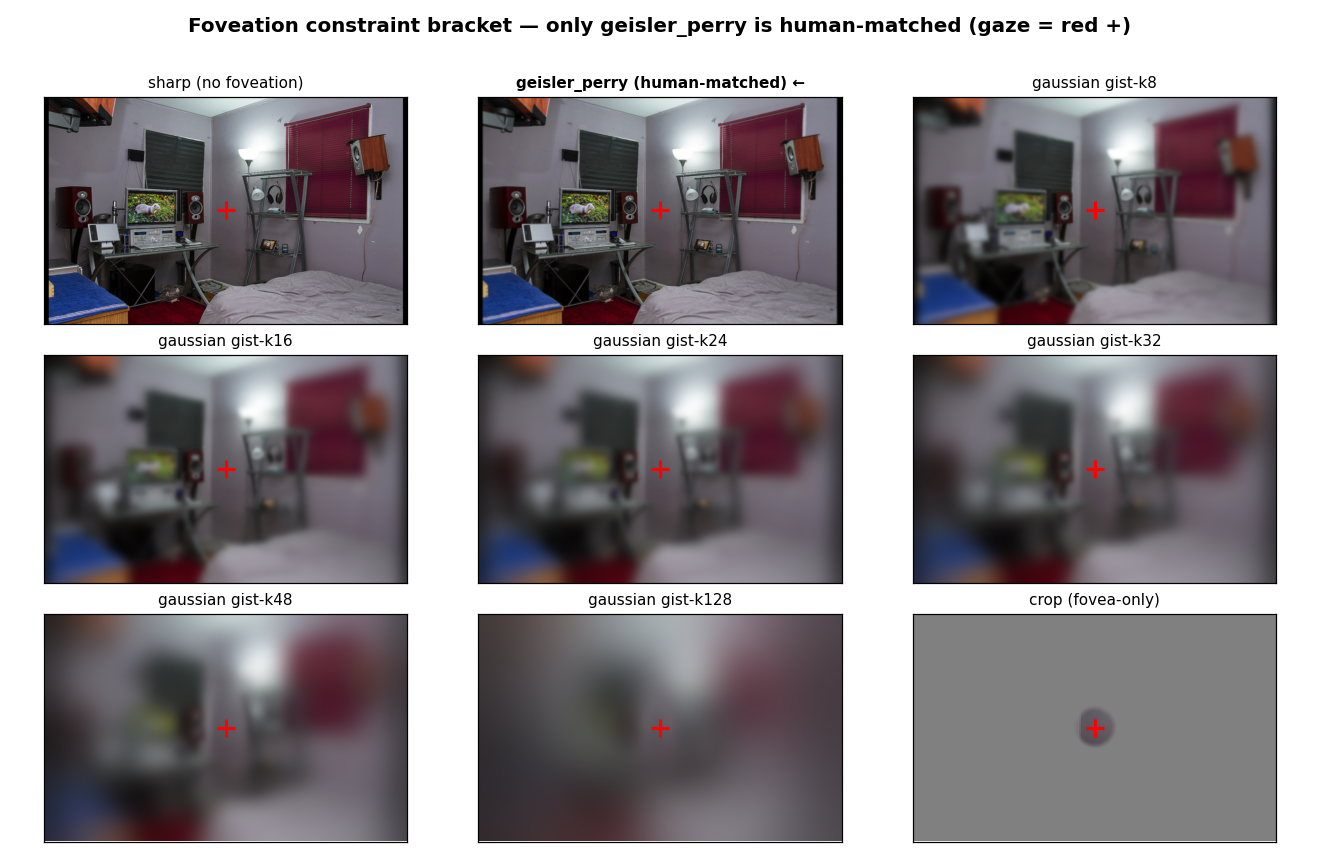
\includegraphics[width=0.58\linewidth]{figures/bracket_all.png}
  \caption{The foveation bracket applied to one scene at a fixed gaze point (red $+$). Only
  \textsc{geisler--perry} is human-matched, and at this geometry it is mild, nearly indistinguishable
  from \textsc{sharp}; the gaussian gist ladder and \textsc{crop} are synthetic anchors.}
  \label{fig:bracket}
\end{figure}
 
  \vspace{-5mm}
\section{Results}
 \vspace{-3mm}
The three models were evaluated on \NImages\ scenes, \NSeeds\ seeds and nine conditions
($3$ models $\times$ \NImages\ scenes $\times$ \NSeeds\ seeds $\times$ nine conditions $=$ \NEpisodes\ episodes), all completed (Sec.~S10). Quantities are reported
at the human-matched GP condition unless a sweep is specified; complete per-condition tables for all three
models appear in the supplement.

  \vspace{-5mm}
\subsection{Decision and finding: models match or exceed humans}
\label{sec:dec}
 \vspace{-3mm}

\begin{table}[!tb]\centering
\caption{Outcome by foveation condition (existence-passed trials); each entry is Qwen/GLM/Gemma (Q/G/Gm) against the human reference (first row; per-model $n$ differs slightly). Finding and outcome measures match or exceed the human values; the \emph{dynamic} gaze divergence is quantified in Table~\ref{tab:gaze}, though target-absent search length (NFix-TA) also differs from humans for Qwen. TFP@$1$/TFP-end: target fixated on the first / by the final saccade (TP); NFix-TP/-TA: median fixations on target-present/absent trials; TA decl.-abs: target-absent declared-absent rate; dens.\ CC: correlation of model and human fixation-density maps.}
\label{tab:outcome}
\setlength{\tabcolsep}{4pt}
\resizebox{\linewidth}{!}{\begin{tabular}{l *{18}{c}}
\toprule
& \multicolumn{3}{c}{TFP@1} & \multicolumn{3}{c}{TFP-end} & \multicolumn{3}{c}{NFix-TP}
& \multicolumn{3}{c}{NFix-TA} & \multicolumn{3}{c}{TA decl.-abs} & \multicolumn{3}{c}{dens.\ CC} \\
\cmidrule(lr){2-4}\cmidrule(lr){5-7}\cmidrule(lr){8-10}\cmidrule(lr){11-13}\cmidrule(lr){14-16}\cmidrule(lr){17-19}
condition & Q & G & Gm & Q & G & Gm & Q & G & Gm & Q & G & Gm & Q & G & Gm & Q & G & Gm \\
\midrule
\textbf{human} & \multicolumn{3}{c}{\textbf{0.49}} & \multicolumn{3}{c}{\textbf{0.93}}
& \multicolumn{3}{c}{\textbf{3}} & \multicolumn{3}{c}{\textbf{5}}
& \multicolumn{3}{c}{---} & \multicolumn{3}{c}{---} \\
\midrule
sharp                  & 0.97 & 0.97 & 0.80 & 0.97 & 0.98 & 0.93 & 2 & 2 & 3 & 1 & 4 & 6 & 0.94 & 0.91 & 0.96 & 0.55 & 0.54 & 0.49 \\
\textbf{GP} & 0.97 & 0.97 & 0.80 & 0.98 & 0.98 & 0.93 & 2 & 2 & 3 & 1 & 4 & 5 & 0.93 & 0.91 & 0.96 & 0.58 & 0.63 & 0.50 \\
k8                     & 0.93 & 0.84 & 0.64 & 0.95 & 0.89 & 0.86 & 3 & 2 & 3 & 2 & 4 & 6 & 0.84 & 0.77 & 0.81 & 0.65 & 0.45 & 0.26 \\
k16                    & 0.78 & 0.71 & 0.42 & 0.91 & 0.80 & 0.75 & 3 & 3 & 4 & 4 & 4 & 6 & 0.78 & 0.77 & 0.68 & 0.70 & 0.38 & 0.45 \\
k24                    & 0.56 & 0.49 & 0.28 & 0.81 & 0.65 & 0.65 & 3 & 3 & 6 & 6 & 4 & 6 & 0.72 & 0.68 & 0.58 & 0.74 & 0.46 & 0.29 \\
k32                    & 0.42 & 0.33 & 0.19 & 0.71 & 0.53 & 0.59 & 3 & 3 & 6 & 7 & 4.5 & 7 & 0.62 & 0.65 & 0.52 & 0.70 & 0.43 & 0.26 \\
k48                    & 0.28 & 0.18 & 0.10 & 0.56 & 0.36 & 0.47 & 5 & 4 & 6 & 7 & 4 & 7 & 0.46 & 0.65 & 0.54 & 0.49 & 0.33 & 0.25 \\
k128                   & 0.15 & 0.09 & 0.01 & 0.31 & 0.22 & 0.39 & 6 & 4 & 6 & 6 & 4 & 6 & 0.85 & 0.86 & 0.78 & 0.18 & 0.14 & 0.19 \\
crop                   & 0.04 & 0.04 & 0.00 & 0.20 & 0.11 & 0.16 & 3 & 3 & 5 & 2 & 3 & 5 & 0.68 & 0.50 & 0.67 & 0.25 & 0.11 & 0.15 \\
\bottomrule
\end{tabular}}
 \vspace{-2mm}
\end{table}
\textbf{Decision.} One-shot present-target detection is near-ceiling and comparable across models (target-present /
target-absent existence accuracy \QwenTPexist/\QwenTAexist, \GlmTPexist/\GlmTAexist,
\GemmaTPexist/\GemmaTAexist; false-positive bias on absent scenes
\QwenYesBias/\GlmYesBias/\GemmaYesBias), so subsequent search divergences cannot be attributed to
detection failure and the existence-passed sets are comparable. In the agentic task the present/absent
decision is highly sensitive for every model ($d'$ \QwenGPDprime/\GlmGPDprime/\GemmaGPDprime, against the
human \HumanDprime; Sec.~S4), and absent scenes are declared absent at \QwenGPDeclAbs/\GlmGPDeclAbs/\GemmaGPDeclAbs\ --- distinct from the one-shot existence accuracy ($\sim$$0.80$) reported above. \textbf{Finding.} Every model fixates the target on the
first saccade far more often than humans (TFP@1 \QwenGPTFPone/\GlmGPTFPone/\GemmaGPTFPone\ against
\HumanTFPone; Table~\ref{tab:outcome}) and attains comparable eventual success (TFP-end
\QwenGPTFPend/\GlmGPTFPend/\GemmaGPTFPend\ against \HumanTFPend), while issuing no more fixations than
humans (median \QwenGPNumFixTP/\GlmGPNumFixTP/\GemmaGPNumFixTP\ against \HumanNumFixTP). On the two axes
of principal practical interest, whether the decision is correct and whether the target is found, the
models are therefore human-or-better; assessed at the level of outcomes alone, they would be judged
human-like. One target-absent behaviour is, however, already non-human on the search axis: Qwen3.5-35B-A3B declares absence after a single fixation (NFix-TA \QwenGPNumFixTA) versus the human median \HumanNumFixTA, an efficiency win that is itself not human-like.
 


\vspace{-5mm}
\subsection{Gaze dynamics: a shared, non-human signature}
\label{sec:gaze}
 \vspace{-1mm}
Under the conditions in which outcomes coincide with humans, the eye-movement \emph{process} does not, and
the deviation has the same direction for all three models (Table~\ref{tab:gaze}, Fig.~\ref{fig:gistpca}b).
Gaze entropy lies below the human value (Cliff's $\delta$ \QwenGPEntropyD/\GlmGPEntropyD/\GemmaGPEntropyD),
indicating spatially concentrated sampling, and saccade amplitudes exceed it
(\QwenGPSaccD/\GlmGPSaccD/\GemmaGPSaccD), indicating direct movements to the target. The scanpaths are
moreover highly self-consistent: cross-seed (agent$\leftrightarrow$agent) ScanMatch is
\QwenGPSelfConsist/\GlmGPSelfConsist/\GemmaGPSelfConsist, far above the human$\leftrightarrow$human
agreement ceiling (\HumanCeiling), so each model reproduces its own scanpath more closely than two humans
agree. A principal-component analysis of the five-statistic signature places all three models, under the
legible conditions, in a region disjoint from the human reference (Fig.~\ref{fig:gistpca}b). That three
unrelated models occupy the \emph{same} region is the multivariate expression of the gaze divergence. These effects survive per-metric mixed-effects models with crossed scene and rater random intercepts (gaze entropy and saccade amplitude have $95\%$ intervals excluding zero for all three models; Sec.~S9).
 
\begin{table}[!tb]\centering
\caption{Gaze axis at the human-matched condition: Cliff's $\delta$ against the human distribution
($|\delta|>0.33$ in bold; sign is agent $-$ human) and cross-seed self-consistency. The deviation is non-human and shares a
common direction across models (sub-threshold for Gemma-4-E4B on entropy and amplitude), whereas center
bias, the spatial prior, is human-like (sub-threshold) for all three. Full seven-statistic Cliff's $\delta$ (all conditions): Table~S3.}
\label{tab:gaze}
\begin{tabular}{lcccc}
\toprule
 & gaze entropy $\delta$ & saccade amp $\delta$ & center bias $\delta$ & agent$\leftrightarrow$agent self-consist. \\
\midrule
human$\leftrightarrow$human ceiling & --- & --- & --- & 0.53 \\
Qwen3.5-35B-A3B & \textbf{$-$.67} & \textbf{$+$.50} & $-$.18 & 0.84 \\
GLM-4.6V-Flash & \textbf{$-$.65} & \textbf{$+$.61} & $-$.31 & 0.91 \\
Gemma-4-E4B & $-$.27 & $+$.23 & $+$.06 & 0.71 \\
\bottomrule
\end{tabular}

 \vspace{-5mm}
\end{table}
 
\subsection{No regime recovers human-like search; a single-pass account}
Sweeping the synthetic degradation does not yield a level at which a model searches like a human (TFP@1
$\approx$ \HumanTFPone) while still locating the target (TFP-end $\approx$ \HumanTFPend). For none of the
three models (Fig.~\ref{fig:gistpca}a) do these quantities separate: they decline together, so by the
degradation that lowers first-saccade targeting to the human rate ($k{=}32$ for Qwen3.5-35B-A3B,
TFP@1/TFP-end \QwenKthirtytwoTFPone/\QwenKthirtytwoTFPend; $k{=}16$ for Gemma-4-E4B,
\GemmaKsixteenTFPone/\GemmaKsixteenTFPend), eventual success has already collapsed. The divergence is
not an effect of acuity: the human-matched condition is behaviourally indistinguishable from \textsc{sharp}
for every model (e.g.\ TFP@1 \QwenGPTFPone\ against \QwenSharpTFPone; Tables~\ref{tab:outcome}--\ref{tab:gaze}),
even though it measurably degrades the periphery. Nor is it a difference of spatial prior: center bias is human-like for all three (sub-threshold $\delta$, Table~\ref{tab:gaze}), so the models look in broadly human-relevant places, whereas the order and dynamics of their fixations (low entropy, large saccades, high determinism) do not. The missing component is serial sampling, not the spatial prior; we do not manipulate architecture directly, so this attribution is by elimination (acuity and spatial prior ruled out) and a causal test imposing serial sampling is left to future work. As evidence is removed the models do not lengthen search gracefully: refixation rises, then at the most severe degradation the declared-absent rate rebounds as they default to absent, a model-internal failure signature needing no human reference (Sec.~S8).
 
\begin{figure}[!tb]
  \begin{subfigure}{0.5\linewidth}\centering
    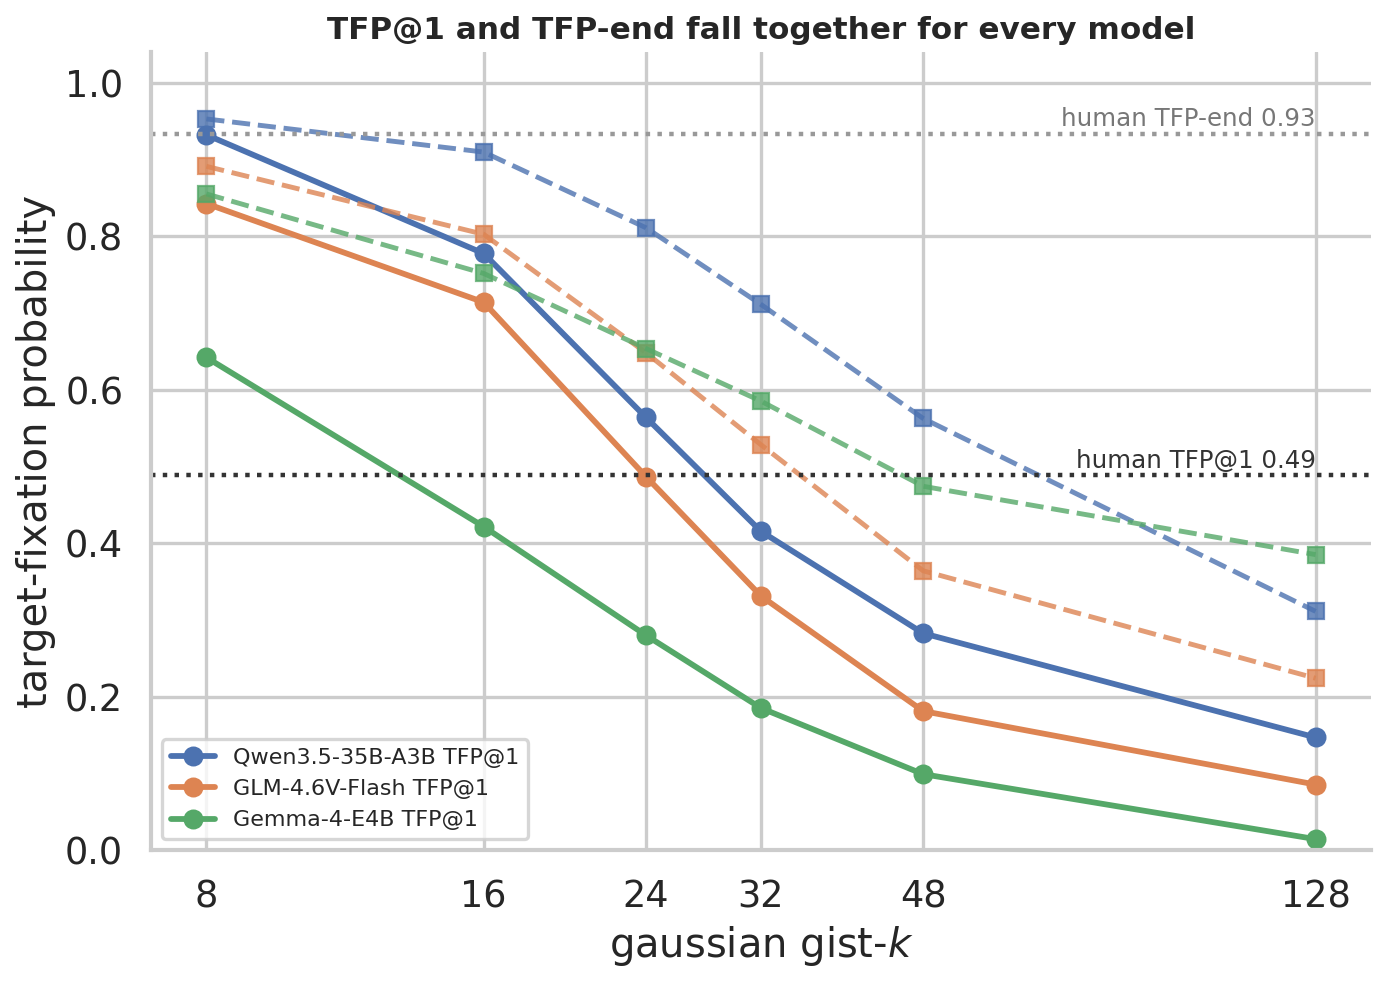
\includegraphics[width=0.80\linewidth]{figures/fig_gist.png}\caption{No human-like regime.}\label{fig:gist}
  \end{subfigure}\hfill
  \begin{subfigure}{0.49\linewidth}\centering
    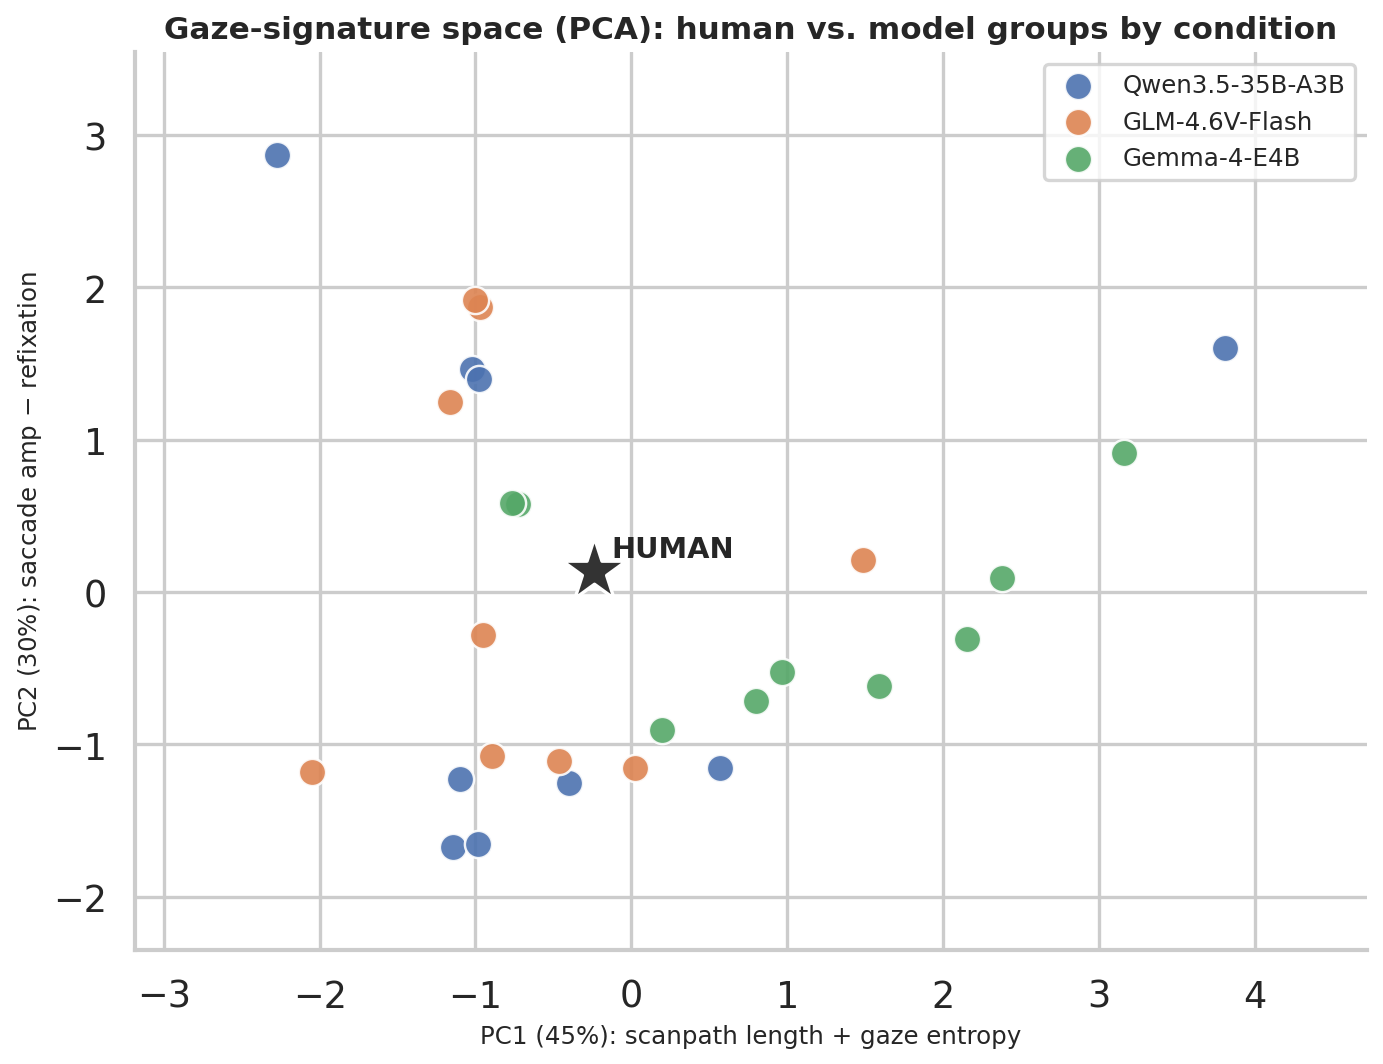
\includegraphics[width=0.80\linewidth]{figures/fig_pca.png}\caption{Gaze-signature PCA (per group).}\label{fig:pca}
  \end{subfigure}
  \caption{(\subref{fig:gist}) First-saccade targeting (solid) and eventual success (dashed) as functions
  of the degradation factor $k$ for the three models, with human reference levels; the two quantities fall
  together, so no $k$ yields human-like search at human-like success. (\subref{fig:pca}) Principal-component
  analysis of the per-(model,\,condition) five-statistic gaze signature (PC1, \PCApcone\%: scanpath length
  and gaze entropy; PC2, \PCApctwo\%: saccade amplitude versus refixation). Under the legible conditions each
  model sits in a region offset from the human reference ($\star$); points approach the human only under
  severe degradation, with Gemma-4-E4B nearest.}
  \label{fig:gistpca}
  \vspace{-7mm}
\end{figure}

 \vspace{-5mm}
\subsection{Generality and robustness}
The dissociation and the shared gaze signature hold across three distinct model families, suggesting a
property of the foveated-MLLM paradigm rather than of a single instance. The
first-saccade advantage holds within every eccentricity-by-size difficulty stratum (Sec.~S9) and is
insensitive to the target-box tolerance: across tolerances of $0.5$, $1$ and $1.5°$, TFP@1 shifts by at
most $\sim$$0.1$. The high cross-seed determinism is not an artifact of low-temperature decoding; in a
temperature sweep on our anchor model (Qwen3.5-35B-A3B) it remains well above the inter-observer ceiling even at
temperature $1.0$ on the legible conditions (Sec.~S9). Cross-seed and human inter-observer agreement are not identical constructs (no matched human intra-observer baseline exists in COCO-Search18), so we treat the determinism gap as suggestive, resting it on this temperature-$1.0$ persistence. The \emph{magnitude} of the gaze deviation follows a consistent ordering across models: Gemma-4-E4B is the most human-like model, with the smallest effect on five of the seven statistics (entropy, saccade amplitude, scanpath length, center bias, coverage; e.g.\ gaze-entropy $\delta$ \GemmaGPEntropyD\ vs.\ Qwen \QwenGPEntropyD; cross-seed ScanMatch \GemmaGPSelfConsist\ vs.\ \QwenGPSelfConsist), and its number of fixations (search extent) is the only fixed effect whose mixed-effects $95\%$ interval contains zero (Sec.~S9). Because architecture, recipe and sparsity covary across three models, we read this as weaker single-pass targeting, not a more human-like strategy, and report it descriptively.
 
 \vspace{-5mm}
\section{Discussion}
\paragraph{Metrics and surrogacy.} The models match the present/absent answer and partially match the
human saliency map (density correlation \QwenGPDensityCC/\GlmGPDensityCC/\GemmaGPDensityCC) yet diverge on
every temporal measure of gaze. Because answer-alignment and saliency scores are computed on outcomes or a
time-collapsed map, a high value is necessary but not sufficient: zero-shot MLLMs are adequate surrogates
for \emph{outcome and spatial} questions but not \emph{process and temporal} ones, a property of the class
that model selection does not remove.
 
\paragraph{A non-human searcher as a null model.} Conversely, a system attaining human-or-better outcomes
\emph{without} a serial bottleneck is a useful null: it isolates the behaviours due to seriality from the detection and spatial priors it
already reproduces.
 
 
\vspace{-5mm}
\section{Limitations and scope}
\label{sec:lim}
Our scope is general-purpose models under a fixed foveation constraint: search-trained agentic,
pointing-native and frontier closed-source models---the most pertinent next comparison---are not evaluated.
The cross-model trend is confounded (architecture, recipe, sparsity) and reported descriptively; the gaze
signature is measured under a single prompt whose memory clause may partly shape refixation; and fixation
durations are human-only.
 
 \vspace{-2mm}
\section{Conclusion}
Under human-matched foveation, three MLLMs match or beat humans on decision and finding yet share \emph{one} non-human gaze signature that no degradation regime makes human-like, the mark of a single-pass architecture with a human-like spatial prior. This \emph{process} axis, which answer-alignment and saliency metrics miss, bounds MLLMs as human-vision surrogates and yields a null model for the serial bottleneck.

\bibliographystyle{splncs04}
\bibliography{main}

\end{document}
